%%%%%%%%%%%%%%%%%%%%%%%%%%%%%%%%%%%%%%%%%%%%%%%%%%%%%%%%%%%%%%%%%%%%%%%%%%%%%%
%
% Main content starts here
%
%%%%%%%%%%%%%%%%%%%%%%%%%%%%%%%%%%%%%%%%%%%%%%%%%%%%%%%%%%%%%%%%%%%%%%%%%%%%%%


\chapter{Introduction}
\label{sec:introduction}

\chapter{Hintergrund und verwandte Arbeiten}
\section{Relevante Konzepte und Definitionen}
\subsection{Deepfakes}
"Deepfakes - Wenn man Augen und Ohren nicht mehr trauen kann" \cite{bildungDeepfakesWennMan2023} - 
So steigt Journalist und Autor der Bundeszentrale für politische Bildung Tim Walter in seinem Artikel über die Gefahren von Deepfakes ein. 
Dies ist nur eins von vielen Beispielen (Weitere Beispiele im Fußbereich) das zeigt, 
dass Deepfakes mittlerweile ein ernstgenommenes Thema in der nicht-technischen Medienwelt und Gesellschaft sind. 
Doch was genau sind eigentlich Deepfakes? 

\textcite{gambinDeepfakesCurrentFuture2024} beschreiben das Konzept Deepfake als "generation of fake digital content or manipulated of genuine one through the use of DL techniques." \cite[S. ?]{gambinDeepfakesCurrentFuture2024},
also frei übersetzt als die Erzeugung von gefälschten digitalen Inhalten oder die Manipulation echter Inhalte durch den Einsatz von Deep Learning Techniken. 
Deep Learning ist ein Teilgebiet der Künstlichen Intelligenz, genauer gesagt des Machine Learning, in dem es darum geht, mithilfe einer Reihe von Methoden automatisch Muster in Daten zu erkennen und diese zur Vorhersage zukünftiger Daten oder Entscheidungen zu verwenden \autocite[S. 1]{murphyMachineLearningProbabilistic2012} . 
Weiter schreiben Gambin et. al "The content inlcudes video, image, audio, and text among other sources." 
In einer ähnlichen Definition heißt es, dass bei Deepfake Videos in den meisten Fällen in einem schon existierenden Video das Abbild einer Person über den Körper einer anderen Person gelegt wird. 
Dadurch sieht es aus, als würde die Person dessen Abbild darüber gelegt wurde die Aktivitäten der anderen Person ausführen \autocite{harrisVideoDemandWhat2021}.
Währenddessen teilen \textcite{juefei-xuCounteringMaliciousDeepFakes2022} Deepfakes in die vier Kategorien "(i) entire face synthesis, (ii) attribute manipulation, (iii) identity swap, and (iv) expression swap (i.e., reenactment)". 
Schon an diesen Beispielen lässt sich erkennen, dass Deepfakes in unterschiedlichen Formen vorkommen.

Nachdem nun geklärt ist, was Deepfakes eigentlich sind, fehlt noch wo Deepfakes ihren Ursprung \cite{AIAssistedFakePorn2017} haben. 
Dazu schreiben \textcite{kernerPornDiscreditationEpistemic2021} "Deepfakes got started in 2017 [...] when an eponymous Reddit user enlisted open-source software from Google and elsewhere to apply scattered academic research to face-swapping". 
Die erste mediale Berichterstattung folgte im Dezember 2017 durch den Artikel \textcite{AIAssistedFakePorn2017} im Vice Tech Magazin Motherboard von Samantha Cole.
Seitdem nimmt die Verbreitung von Deepfakes immer weiter zu, was man unter anderem bei \textcite{ranaDeepfakeDetectionSystematic2022,westerlundEmergenceDeepfakeTechnology2019,gamagePDFEmergenceDeepfakes} sieht. 
Auch die Google Suchtrends zum Keyword "Deepfake" bestätigen diese Aussage, siehe Grafik \ref{fig:suchtrend-grafik}.
\begin{figure} [htbp]
    \centering
    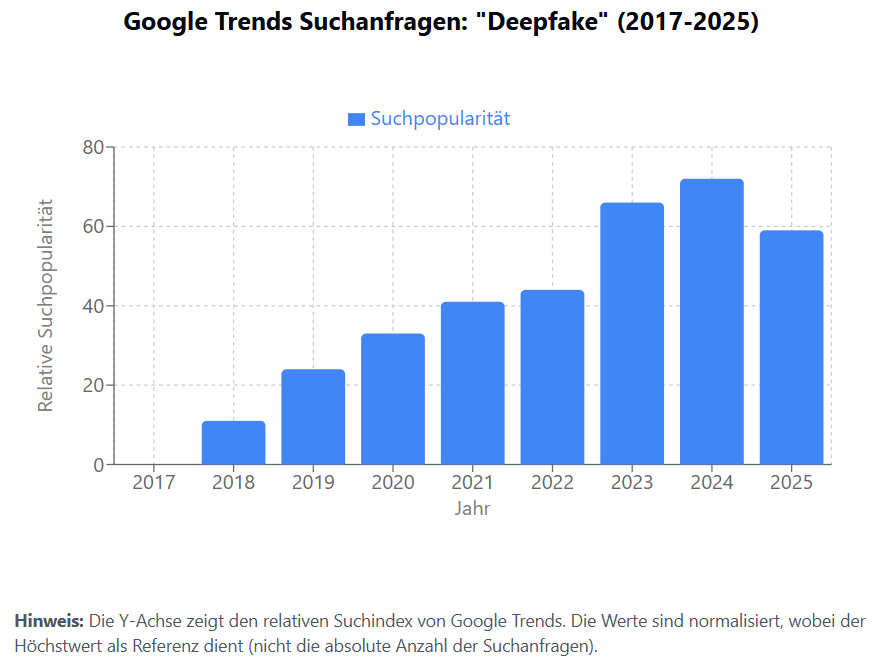
\includegraphics[width=0.8\textwidth]{GrafikGoogleTrendDeepfake.png}
    \caption{Google Suchtrend zum Keyword "Deepfake"}
    \label{fig:suchtrend-grafik}
\end{figure}

Seitdem werden Deepfakes allerdings auch immer wieder für negative Zwecke eingesetzt. 
Ein großer Einsatzbereich und auch der Ursprung von Deepfakes ist die Pornographie \autocite{ajderDeeptraceLabReport}. 
Aber auch abseits von Pornographie gibt es noch mehr kriminelle oder bösartige Einsatzbereiche von Deepfakes. 
Darunter sind unter anderem "spreading misinformation, creating political instability, or various cybercrimes" \cite{ranaDeepfakeDetectionSystematic2022} 
oder wie \textcite{gambinDeepfakesCurrentFuture2024} die Konsequenzen von Deepfakes als "far reaching, including the potential to ignite political or religous tensions between nations, decieve the public, disrupt financial markets, perpetrate acts of sabotage, fraud, scams, obstruct justice, and much more" beschreiben.
Im Folgenden einige Beispiele aus der Praxis von Fällen in denen Deepfakes mit krimineller oder bösartiger Absicht eingesetzt wurden.
\begin{itemize}
    \item Manipulation in der Politik: Ein Audio-Deepfake in dem der slowakische Spitzenkandidat Michal Šimečka scheinbar mit einer 
        Journalistin über das Kaufen von Wählerstimmen diskutiert, wird kurz vor der Parlamentswahl im Oktober 2023 veröffentlicht. 
        Dieser Deepfake wurde strategisch kurz vor der Wahl platziert und durch die slowakische Regelung, 
        dass 48 Stunden vor der Wahl in den Medien kein Wahlkampf mehr betrieben werden darf, wurde eine Richtigstellung noch erschwert. \autocite{pawelecPolitischeManipulationUnd2024}
    \item Revenge Porn und andere nicht-einvernehmliche Inhalte: 
        Im Fall von Hannah Grundy wurden Deepfake Fotos mit pornographischen Inhalten von ihr auf einer Website "The destruction of Hannah" hochgeladen \autocite{WomansDeepfakeBetrayal2025}.
        In einem anderen Fall wurde im türkischen Wahlkampf ein Deepfake Video mit pornographischem Inhalt von Kandidat Muharrem İnce veröffentlicht, 
        was dessen Rücktritt aus dem Wahlkampf zur Konsequenz hatte. \autocite{TurkishPresidentialCandidate2023}
    \item Verleumdung von bekannten Persönlichkeiten: Prominente Personen werden regelmäßig Opfer von Deepfakes, 
        die ihren Ruf schädigen sollen oder Produkte in ihrem Namen ohne ihre Zustimmung bewerben \autocite{PDFImpactDeepfake2025}.
    \item Manipulierte Unternehmenskommunikation: Durch gezielte Deepfakes können Angestellte oder Aktionäre getäuscht und betrogen werden \autocite{PDFImpactDeepfake2025}.
\end{itemize}
Bei all den negativen Beispielen ist zu beachten, dass die Deepfake Technologie an sich neutral ist und auch vielfache Weise positiv eingesetzt werden kann. Im Folgenden einige positive Beispiele wie Deepfakes eingesetzt werden können \autocite{westerlundEmergenceDeepfakeTechnology2019}:
\begin{itemize}
    \item Filmindustrie: Das Erzeugen der Stimmen von Schauspielern die ihre Stimme wegen einer Krankheit verloren haben. 
        In einem anderen Fall hat 2019 eine Malaria Kampagne David Beckham durch Deepfake Technologie multilingual wirken lassen um möglichst viele Menschen ansprechen zu können.
    \item Medizinischer Bereich: Durch Deepfakes können Alzheimer Patienten mit jüngeren Gesichtern interagieren, die sie möglicherweise wiedererkennen. 
    \item Wirtschaftsbereich: Das digitale Anprobieren von Kleidung kann durch Deepfake Technologie ermöglicht werden.
\end{itemize}
Diese Beispiele zeigen, dass die Deepfake Technologie jetzt schon in der Gesellschaft verankert ist, und sich in Zukunft noch weiter ausbreiten wird.

\subsection{Public Displays}
In Krankenhäusern, Universitäten, Bahnhöfen oder Shopping Center. 
An immer mehr öffentlichen oder halb-öffentlichen Orten findet man mittlerweile interaktive Bildschirme, 
nachfolgend auch "Public Displays" genannt. Nach \textcite{parkerDoesPublicStill2018} ist ein Public Display 
ein "medium that brings digital content into the real world and into the eyes of the general public." \cite{parkerDoesPublicStill2018} 
Waren es früher noch nur große Bildschirme die Werbung, Videos oder andere Informationen ohne Möglichkeit zur Interaktion angezeigt haben \cite{PDFEnticingPeople}, 
werden diese heute immer mehr eingesetzt um Informationen visuell und vor allem oft interaktiv darzustellen \cite{hinrichsInteractivePublicDisplays2013}. 
Beispiele aus eigener aktueller (Mai 2025) Erfahrung von Public Displays sind die interaktiven Bildschirme im Münchner Olympia-Einkaufszentrum, 
mit deren Hilfe Besucher Informationen über die verschiedenen Läden einholen können. 
Ein weiteres Beispiel sind Public Displays in Hauseingängen von Mehrparteienhäusern, 
die von den Hausbewohnern zum Informationsaustausch genutzt werden, aber auch um Informationen von der Hausverwaltung an die Bewohner weitergeben zu können.
Einen Schritt weiter geht die Forschung zu sogenannten "public security user interfaces". 
Diese sind definiert als "any type of interface positioned in shared, 
non-personal areas that offers information or the opportunity to interact with security-related topics" \cite{murtezajPublicSecurityUser2025}. 
Durch die zunehmende Bedrohung von Cyber Angriffen ist die Idee entstanden, mithilfe von Public Displays die öffentliche Wahrnehmung von Sicherheitsthemen zu erhöhen. 
Eingesetzt werden diese Interfaces, um bestimmte Ziele zu erreichen, die im folgenden kurz vorgestellt werden.
\begin{itemize}
    \item Creating Awareness: Das Ziel ist, die Nutzer auf mögliche Sicherheitsrisiken aufmerksam zu machen, wie z.B. die Verwendung desselben Passworts für verschiedene Plattformen.
    \item Triggering Actions: Der Nutzer soll dazu gebracht werden, direkt eine Aufgabe in Bezug auf einen Sicherheitsaspekt anzugehen. 
        Ein Beispiel wäre, den Nutzer aufzufordern, verfügbare Sicherheitsupdates für sein Gerät zu installieren.
    \item Sparking Conversation: Hier ist das Ziel, durch das Public security user interface eine Diskussion über bestimmte Sicherheitsthemen anzustoßen, 
        beispielsweise durch fun facts oder andere gesprächsanregende Informationen. 
        Dadurch soll das Thema der Cyber Security noch mehr in den Alltag integriert werden.
\end{itemize}
Diese Ziele geben jetzt schon zahlreiche Einsatzmöglichkeiten und lassen Raum für weitere \cite{murtezajPublicSecurityUser2025}.

\section{Bestehende Technologien}
\subsection{Erzeugung von Deepfakes}
Nachdem nun bekannt ist, was Deepfakes eigentlich sind und wo diese ihren Ursprung haben, wollen wir nun klären wie diese erzeugt werden.
Die ersten Deepfake Videos wurden wie schon beschrieben 2017 von einem anonymen Reddit User erstellt, 
der mit verschiedenen Open-Source Programmen frühe face-swapping Algorithmen aus der Forschung angewandt hat \cite{kernerPornDiscreditationEpistemic2021}. 
Ausführlicher beschreibt es nur \textcite{AIAssistedFakePorn2017} in ihrem Artikel für das Vice Tech Magazin Motherboard. 
Demnach hat der Reddit User "deepfakes" mithilfe von verschiedenen Open-Source Bibliotheken wie Keras und Trainingsbildern aus Google Bilder, 
Stock Fotos und Youtube Videos einen Algorithmus trainiert, der dann in die entsprechenden Vorlagen Videos die Gesichter der Prominenten Personen einfügt \cite{AIAssistedFakePorn2017}.
Eine Technologie mit großen Fortschritten in der Erzeugung von Deepfake Inhalten ist das Modell der sogenannten "generative adversarial networks", 
eingeführt durch \textcite{goodfellowGenerativeAdversarialNetworks2014}, nachfolgend auch GANs genannt. 
Diese GANs bestehen aus zwei neuronalen Netzwerken, dem Generator und dem Discriminator. 
Diese zwei Teile werden gleichzeitig trainiert, wobei der Generator das Ziel hat, den Discriminator mit möglichst echt wirkenden Bildern zu täuschen, 
und der Discriminator das Ziel hat, sich nicht von dem Generator täuschen zu lassen \cite{benaissaOverviewGANDeepFakesDetection2024}. 
Weiterhin gibt es mittlerweile eine Menge von verschiedenen GAN Modellen die zur Erzeugung von Deepfakes genutzt werden. 
Eine Auswahl davon stellt \textcite{benaissaOverviewGANDeepFakesDetection2024}vor, darunter sind DCGAN, CycleGAN, PGGAN und einige mehr.

Im Bereich der Bilderzeugung ist mittlerweile das Modell der Diffusion Modells zum Standard geworden \cite{guptaPhotorealisticVideoGeneration} 
und hat die vorher beschriebenen GANs übertroffen \cite{williampeeblesScalableDiffusionModels}. 
Ein Model zur vollständig künstlichen Erzeugung von Deepfakes, welches zum Zeitpunkt des Schreibens für einige Schlagzeilen \cite{proschofskyGooglesNeueVideoKI2025} gesorgt hat, 
ist das video generation Model Veo 3 von Googles Deepmind. Dieses verwendet ein latent diffusion model (veo 3 tech report). 
Ein Diffusion Model lernt Bilder zu erstellen, indem es aus einem Bildrauschen schrittweise das Rauschen immer weiter entfernt \cite{guptaPhotorealisticVideoGeneration}. 
Dieses wird außerdem in einem latent space angewendet. Statt direkt auf den Pixeln zu arbeiten, 
lässt man das Model in einem "lower-dimensional latent space" \cite{guptaPhotorealisticVideoGeneration} arbeiten, was den Rechenaufwand deutlich reduziert. 
Hierfür lässt man einen Autoencoder Bilder in kleinere räumliche Repräsentationen komprimieren und das diffusion model auf diesen räumlichen Repräsentationen trainieren. 
Einige Beispiele zu was Veo 3 fähig ist, sieht man auf Googles Deepmind Youtube Channel \cite{Veo3Our}.

\subsection{Technische Gegenmaßnahmen für Deepfakes}
Je besser das Erzeugen von Deepfakes wird, desto schwieriger werden auch die Gegenmaßnahmen zu Deepfakes. 
Hierzu gibt es auf der technischen Seite unterschiedliche Herangehensweisen, welche in aktive und passive Maßnahmen eingeteilt werden können, 
wobei sich diese generell noch in frühen Stadien befinden \cite{abbasUnmaskingDeepfakesSystematic2024}.
\subsubsection{Erkennung}
Die passive Herangehensweise ist das klassische Erkennen von deepfakes durch Technologien die selbst auf machine learning oder sogar deep learning basieren. 
Das Literature Review von Abbas und Taeihagh zeigt hier eine Vielzahl von deep learning Technologien, 
darunter eine Menge Varianten die auf CNNs basieren, aber auch eine einige Varianten die auf den oben vorgestellten GANs basieren. 
\textcite{benaissaOverviewGANDeepFakesDetection2024} zeigen noch zwei weitere interessante Ansätze speziell für die Erkennung von deepfake Videos. 
Der eine ist die "biological signal analysis". Bei diesem werden physiologische Signale wie Blinzeln, Augenbewegung oder Herzschlag analysiert und damit die Videos auf Echtheit überprüft. 
In einem Fall wurde dafür eine Kombination aus einem convolutional neural network und einem recursive neural network verwendet, 
ein einem anderen Fall wurden auch wieder die oben genannten GANs verwendet.
Der andere Ansatz ist die "spatial and temporal features analysis". Bei diesem wird nicht wie bei den meisten anderen Ansätzen mit einzelnen Video Frames gearbeitet. 
Hier werden zeitliche und räumliche Merkmale über den Verlauf des Videos mit verschiedenen Modellen wie GANs oder CNNs analysiert und damit auf Echtheit geprüft \cite{benaissaOverviewGANDeepFakesDetection2024}.
\subsubsection{Authentifizierungssysteme}
Um aktiv gegen Deepfakes vorzugehen, bietet sich die Authentifizierung von echten Videos an, 
ein sogenanntes "Proof of Authenticity System" \cite{gambinDeepfakesCurrentFuture2024}. 
Hier konzentriert sich die Forschung vor allem auf blockchain basierte Technologien um echte Videos zu verifizieren. 
Diese funktionieren durch ein dezentrales Transaktionssystem, 
welches durch seine Eigenschaften nahezu fälschungssicher ist und Transaktionen allgemein sicherer und transparenter macht \cite{gambinDeepfakesCurrentFuture2024}. 
Die Idee dahinter ist, Inhalte und im speziellen Videos und Bilder bis zu ihrem Ersteller zurückverfolgen zu können, 
mitsamt wichtigen Metadaten wie Aufnahmezeitpunkt, Kameramodell und andere Logs. 
Durch die Möglichkeit, die Inhalte bis zu ihrem Ersteller zurückverfolgen zu können, sollen diese vertrauenswürdig und "authentisch" sein.
\section{Verwandte Arbeiten und Stand der Forschung}
\subsection{Menschliche Deepfake Erkennung}
Eine nicht zu vernachlässigende Frage ist, ob auch Menschen in der Lage sind, Deepfake Inhalte zuverlässig zu erkennen. 
\textcite{dielHumanPerformanceDetecting2024} versuchen diese Frage in ihrem Review zu beantworten. 
Ohne Training liegt die menschliche Erkennung von Deepfake Inhalten auf dem gleichen Level wie Raten. 
Um diese zu verbessern, gibt es einige Ansätze \cite{dielHumanPerformanceDetecting2024}:
\begin{itemize}
    \item "raising awareness": Das Aufmerksam machen der Menschen auf das potentielle Auftreten und die Gefahren von Deepfake Inhalten
    \item "feedback training": Nach der Entscheidung ob ein Stimulus echt war oder nicht, bekommt der Nutzer direktes Feedback, z.b. in Form von positiven oder negativen Feedback
    \item "providing advice": Dem Nutzer werden zusätzlich noch Ratschläge gegeben wie man Deepfake Inhalte besser erkennen kann
    \item "Caricaturization": Das Hervorheben bzw. die übertriebene Darstellung von Deepfake Artefakten durch Karikaturisierung
    \item "support based strategies": Ansätze wie KI-Support oder der Kollaboration der Nutzer in Gruppen
\end{itemize}
Einzeln angewendet bringen diese Ansätze gemischte Ergebnisse hervor. 
Sowohl "raising awareness" als auch "providing advice" bringen nur in manchen Studien signifikante Verbesserungen, 
während hingegen "feedback training", "caricaturization" und "support based strategies" sehr konstant die menschliche Erkennung von Deepfake Inhalten verbessern. 
Aber gerade die Kombination aus mehreren Ansätzen, wie zum Beispiel "feedback training" und "providing advice" könnten noch weitere Verbesserungen bringen \cite{dielHumanPerformanceDetecting2024}. 
Allerdings sollte man Diels Bemerkung, "caution should be taken when attempting to generialize the present results 
as deepfake detection performance may depend on various factors (e.g., deepfake qualitiy)." \cite{dielHumanPerformanceDetecting2024} nicht unerwähnt lassen.
Eine hilfreiche Anleitung zum Erkennen von Deepfake Videos gibt das MIT\cite{ProjectOverviewDetect}.
Basierend auf diesen und mit Eindrücken des Politifact \cite{settlesPolitiFactDemystifiesDeepfake} Artikels sind folgend die Strategien 
die in der Anwendung den Nutzern näher gebracht werden:
\begin{itemize}
    \item Achte auf das Gesicht. Hochwertige DeepFake-Manipulationen zeigen oft subtile Artefakte und Verzerrungen in den Gesichtszügen.
    \item Achte auf die Wangen und die Stirn. Wirkt die Haut zu glatt oder zu faltig? 
        Ist das Alter der Haut ähnlich wie das Alter der Haare und Augen? DeepFakes können in einigen Dimensionen inkongruent sein.
    \item Menschen blinzeln typischerweise alle 4-6 Sekunden. Bei Deepfakes sind die Blinzelmuster oft unnatürlich oder fehlen komplett.
    \item Achte auf die Augen und Augenbrauen. Natürliche Schatten und Bewegungen sind in Deepfakes oft unvollständig oder fehlerhaft dargestellt.
    \item Achte auf Brillenreflexionen. Bei Deepfakes sind Lichtreflexionen oft unnatürlich oder stimmen nicht mit der Szenenbeleuchtung überein.
    \item Achte auf die Gesichtsbehaarung. Deepfakes haben oft Schwierigkeiten, Bart, Schnurrbart oder Koteletten natürlich darzustellen und zu animieren.
    \item Achte auf Leberflecken und Muttermale. Deepfakes haben oft Schwierigkeiten, diese Details konsistent darzustellen oder sie verschwinden komplett zwischen den Frames.
    \item Überprüfe im Zweifelsfall die Authentizität eines Videos, 
        indem du online nach der Quelle und dem Kontext suchst. Verwende vertrauenswürdige Faktenprüfungs-Websites und Rückwärtsbildsuche-Tools.
\end{itemize}
\footnote{Anmerkung: Ursprünglich gab es noch eine Strategie zur Lippensynchronisation. 
Diese wurde allerdings aufgrund des nicht vorhandenen Audio der Videos bewusst entfernt.}
Um diese Strategien überhaupt testen zu können bedarf es auch entsprechenden Videos. 
Hierfür gibt es in der Forschung vorgefertigte Datensätze. 
Eine gute Übersicht gibt die Datensatzübersicht von Papers with Code \cite{PapersCodeMachine}. 
Für diese Arbeit wurde der Celeb-DF Datensatz verwendet. 
Dieser Datensatz besteht immer aus einem echten Video einer prominenten Person und einen Satz an Deepfake Videos die aus dem echten Video generiert wurden.

\subsection{Public Displays als "public security user interfaces"}
Um die beiden oben beschriebenen Punkte Deepfake Erkennung und Public Displays zu verbinden, 
bietet sich das oben beschriebene Konzept der public security user interfaces von an. 
\textcite{murtezajPublicSecurityUser2025} sehen "a strong potential at the intersection of research on interaction in public space and IT security-related behavior change", 
also in der Kombination von public displays und sicherheitsrelevanten Themen wie in unserem Fall Deepfake Inhalten. 
Andere Fälle wo dies in der Praxis bereits angewandt wird sind eher selten. Die Universität Toronto sowie die Firma Rise Vision haben zum cybersecurity awareness Monat spezielle, 
allerdings nicht interaktive, Ressourcen für public displays entwickelt \cite{visionCyberSecurityAwareness,CyberSecurityAwareness}. 
\textcite{daviesOpenDisplayNetworks2012} schlagen vor, public displays zur Unterstützung von Verhaltensänderungen (z.b. "walk-to-school program), 
Support bei Notfallsituationen, oder personalisierten Informationen zu nutzen. 
Ein potentielles Szenario mit direkteren Fokus auf die Cybersecurity zeigen \textcite{murtezajPublicSecurityUser2025} anhand des Beispieles einer fiktiven Firma die mithilfe 
von Public Displays in ihren Räumlichkeiten die Einführung eines Passwortmanagers unterstützen. 

\chapter{Methoden}
Im Folgenden wird beschrieben wie das Spiel entwickelt wurde und welche Anforderungen an das Spiel bestehen.
\section{Anforderungsanalyse}
Dazu wird zuerst auf die Anforderungen eingegangen. 
Es stellen sich die Fragen: Was ist eigentlich das Ziel und der Anwendungskontext? 
Was sind die funktionalen Anforderungen? Was sind die nicht funktionalen Anforderungen?
Das Ziel für diese Arbeit war, eine Anwendung zu schreiben die zusammen mit der für den Nutzer nachfolgenden Umfrage die nötigen Daten und Erkenntnisse hervorbringt, 
um die Forschungsfragen zu beantworten. Dazu wurde ein Spiel benötigt, welches auf einem Public Display läuft, 
den Nutzer vor die Entscheidung stellt ob ein gezeigtes Video echt oder ein Deepfake ist, 
und diesem folgend noch Strategien zur Erkennung von Deepfake Videos an die Hand gibt. 
Dies passiert alles in der Öffentlichkeit bzw. in diesem Fall in einem Durchgangsgebäude der Universität in dem hoher Durchgangsverkehr von Studenten besteht.
Im Detail muss die Anwendung, im nachfolgenden als Spiel bezeichnet, einen Startbildschirm besitzen, der möglichst die Aufmerksamkeit der Passanten auf sich zieht und diese zum Spielen animiert. 
Weiter muss natürlich das Video und der Bildschirm zur Entscheidung ob echt oder Deepfake angezeigt werden. 
Auch von entscheidender Bedeutung ist die Ansicht der oben beschriebenen Strategien zur Erkennung von Deepfake Videos. 
Da das Spiel auf einem Public Display läuft, gibt es keine Möglichkeit dem Nutzer die Funktionen und Steuerung zu erklären. 
Diese müssen deshalb den gängigen User-Experience Konventionen folgen um möglichst selbsterklärend zu sein. 
Außerdem sollte das Spiel zusätzlich zur deutschen Version noch eine Möglichkeit zum Spielen auf Englisch anbieten um auch internationalen Passanten das Spielen zu ermöglichen.

\section{Systemdesign}
Mit Hinblick auf die eben genannten Anforderungen wird nun beschrieben wie das Spiel aufgebaut ist, 
und auf welcher Softwarearchitektur und Technologie das Spiel basiert.
Zusätzlich zu den benötigten Hauptfunktionen, also Startbildschirm, Videoansicht, Entscheidungsansicht und Strategieansicht, gibt es noch folgende Funktionen:
\begin{itemize}
    \item Videovergleichsansicht: Nach der Entscheidung kann der Nutzer sich nochmals beide Videos, also echt und Deepfake, anschauen.
    \item Gründe warum das gezeigte Video Deepfake war, bzw. woran man das Deepfake Video erkennen kann (in der Videovergleichsansicht enthalten).
    \item Statistikansicht: Eine Übersicht mit der Erfolgsrate der Entscheidungen und der Anzahl von schon gesehenen Videos.
    \item Spiel speichern: Der Nutzer hat die Möglichkeit, sich einen 4-stelligen Pin zu erzeugen mit dem er sich zu einem späteren Zeitpunkt wieder einloggen
         und mit seinen bestehenden Statistiken weiter spielen kann (in der Strategieansicht enthalten).
    \item QR-Code Ansicht: Damit wird der Nutzer über einen individuell generierten QR-Code auf die Umfrage weitergeleitet, wodurch sich Spielstatistiken und die Umfrage verknüpfen lassen.
    \item Die Benutzerführung für die Hauptfunktionen erfolgt nach einem Tap auf den Spiel starten Button im Hauptbildschirm durch eine horizontale Navigation. 
        Das bedeutet der Nutzer kann mittels "Swipe" Geste oder seitlichen Buttons in Pfeil-Form von links nach recht durch die Ansichten navigieren. 
        Zu den Zusatzfunktionen Statistik, Spiel speichern und QR-Code gelangt der Nutzer über eine Button Reihe in der Strategieansicht. Für die genaue Benutzerführung siehe Grafik "Userflow".
\end{itemize}
Das Spiel wurde mit dem Cross-Platform Framework Flutter entwickelt, ursprünglich als Webanwendung und letztendlich als native Windowsanwendung. 
Dies zeigt auch eine Stärke von Flutter, die einfache Verwendung auf verschiedenen Plattformen.
Die darunter liegende Softwarestruktur basiert vor allem auf dem BloC-Pattern \cite{BlocStateManagement}, vergleichbar mit dem bekannten MVC-Pattern. 
Hier wird die Logik in drei Ebenen aufgeteilt, die Präsentation, die Geschäfts-Logik und die Datenebene. 
Die Datenebene ist aufgeteilt in die Data Providers, also die Datenquellen, und die Repositories, die aus den rohen Daten verwendbare Objekte machen. \cite{Architecture}
Zur Kommunikation zwischen den Ebenen wird mit Zuständen und Events gearbeitet.
\section{Implementierung} 
Im folgenden wird gezeigt wie das BloC-Pattern und zentrale Funktionen konkret implementiert wurden. 
Die Logik Ebene wird von der GameBloc Klasse implementiert. 
In dieser wird definiert wie konkret auf die verschiedenen Events reagiert wird. 
Die möglichen Events dafür werden in der game event Klasse definiert, die möglichen Spielzustände in der gamestate Klasse.
Die Präsentationsebene wird konkret von den game screens implementiert. 
Diese werden abhängig von dem aktuellen game state angezeigt und rufen bei Nutzereingaben wiederum die definierten Events auf. 
Die Datenebene wird durch die verschiedenen Repositories wie z.b. das user repository oder das video repository koordiniert. 
Dabei bezieht beispielsweise das video repository mithilfe der storage Klasse die Liste mit vorhandenen Videos aus einer Video Datenbank in Form einer json Datei. 
Diese Liste wird dann wie im video model beschrieben in eine Liste mit video Objekten umgewandelt. 
Alles was die Logik Ebene zu sehen bekommt sind dann die generierten Video Objekte. 
Die restliche Datenverarbeitung funktioniert parallel zu diesem Beispiel.
Die persistente Datenspeicherung der Spielerstatistiken erfolgt über die Flutter Bibliothek Hive \cite{IsarHive2025}. 
Besonders hilfreich für die Nutzung im Rahmen der Studie und die Auswertung der Ergebnisse ist das QR-Code Feature. 
Für jeden Spieler wird ein eigener QR-Code generiert, der auf den Link zur Umfrage verweist und zusätzlich eine 6-stellige Referenznummer enthält, 
die gleichzeitig die interne Session-ID für jeden Spieler ist. 
Mit dieser Session-ID können also die Ergebnisse der Umfrage mit den geführten internen Statistiken verknüpft werden. 
Die internen Statistiken beinhalten unter anderem die Anzahl an gespielten Spiele (entspricht der Anzahl an gesehenen Videos), 
Anzahl der korrekten Entscheidungen, ob überhaupt ein Spiel gespielt wurde, die Spieldauer und das initial confidence rating, auf welches später nochmal genauer eingegangen wird.  

Besonders wichtig für die Spieler sind natürlich die Strategien. 
Jede Strategie wird als eigene Karte in einem horizontalen Karussell dargestellt. 
Für jede Strategie kann der Nutzer sich jeweils eine simple Abbildung anschauen, einmal wie der reale Inhalt aussehen würde, und einmal wie der Deepfake Inhalt aussehen würde. 
Die Navigation in dem Karussell erfolgt über horizontale Swipe Gesten. 
ufgrund von eingeschränkter Swipe Funktionalität auf dem Testgerät wurden noch simple Buttons zur Navigation nach links und rechts implementiert.
\chapter{Studiendesign}
\section{Hypthesen}
Um die in der Einführung beschriebenen Forschungsfragen beantworten zu können, werden folgende Hypothesen aufgestellt:
...
\section{Aufbau der Studie}
Die Studie erfolgt als Feldstudie mit einer nachfolgenden optionalen Umfrage und ist in zwei Phasen aufgeteilt. 
In der ersten Phase werden Teilnehmer aktiv angesprochen und zu der Teilnahme an dem Spiel und der Umfrage eingeladen. 
Hierbei gibt es weder Einflussnahme wie gespielt werden soll, noch auf die Spieldauer der Teilnehmer. 
Diese Phase ist auf 4 Tage, jeweils von 10:00 bis 16:00 Uhr angesetzt. 
In der zweiten Phase wird das Spiel ohne Aufsicht und aktives Ansprechen für 8 Tage fortlaufen. 
Die Einteilung in zwei Phasen erfolgt um zuerst sicher zu stellen, dass sich ausreichend Teilnehmer (30-40) für die Studie finden. 
Durch das aktive Einladen der Teilnehmer ist natürlich nicht messbar, ob und wie viele Passanten von sich aus den Public Display nutzen. 
Um dies herauszufinden gibt es dann die zweite Phase der Studie.

Das Setup besteht aus einem 55 Zoll Touchscreen mit angeschlossenem Workstation PC basierend auf Windows 11. 
Aufgebaut ist es in einem Durchgangsraum der LMU München während auch aktiv Vorlesungen in dieser Zeit stattfinden. 
In dem Raum gibt es eine hohen Frequenz an Passanten und Studenten, die in diesem Raum lernen oder Pause machen. 
Das Display steht direkt an dem Korridor den die Passanten durchlaufen und gleichzeitig gut sichtbar im Blickfeld der an den im selben Raum befindlichen Tischen, 
an denen die Studenten sitzen. Mögliche Störfaktoren sind vor allem die zwei temporären Verkaufsstände von Studentenzeitungen und Magazinen. 
Diese könnten potentiell die Aufmerksamkeit der Passanten auf sich und damit weg von dem Public Display ziehen.

Als Hauptzielgruppe der Teilnehmer ergeben sich natürlich vorrangig Studenten, grundsätzlich ist aber ein breites Teilnehmerfeld möglich. 
Einschränkungen an die Teilnehmer gibt es im Grunde keine, vorausgesetzt die Bedienung des Touchscreens ist möglich und der Teilnehmer hat ein Smartphone dabei um die Umfrage auszufüllen. 
Erwartet werden für die erste Phase ca. 30-40 Teilnehmer, für die zweite Phase ist die Anzahl nicht vorhersehbar wobei es theoretisch auch keinerlei Teilnehmer geben kann.

\section{Methoden der Datenerhebung}
Jetzt gilt es noch zu klären wie die Daten und welche Daten eigentlich erhoben werden. 
Auch das passiert zwei geteilt. 
Zum einen werden während der Laufzeit des Spiels interne Statistiken aufgezeichnet und in einer JSON Datei gespeichert. 
Diese umfassen für jeden Spieler folgende für die Auswertung interessante Variablen:
\begin{itemize}
    \item Session ID: übergreifende ID zur Verknüpfung der internen Statistiken und Umfrage
    \item Anzahl gespielter Spiele
    \item Anzahl richtiger "Entscheidungen" (Entscheidung ob spezielles Video real oder Deepfake ist)
    \item Anzahl der Anmeldungen eines Spielers (wie oft hat er sich eingeloggt?)
    \item Boolean "hat mindestens ein Spiel komplett durchgespielt"
    \item Boolean "hat das Spiel gespeichert und einen Pin generiert"
    \item Boolean "hat sich wieder eingeloggt (mit seinem Pin)"
    \item Zeitstempel des ersten Spiels
    \item Zeitstempel des letzten Spiels
    \item "Confidence Rating": Antwort von 1-5 auf die Frage "Wie würdest du deine Fähigkeit einschätzen, Deepfake-Videos zu erkennen?"
\end{itemize}
Der andere Teil der Daten wird über eine Online-Umfrage erfasst. 
Dazu erhalten die Nutzer des Spiels die Möglichkeit nach dem Spielen einen QR-Code abzuscannen, der zu der Umfrage führt. 
Der Fragebogen steht auf Deutsch und Englisch zu Verfügung, im folgenden eine Übersicht der deutschen Fragen mit den Antwortmöglichkeiten:

\begin{enumerate}
    \item Confidence Check: Frage "Wie würdest du deine Fähigkeit (nach dem Spielen) einschätzen, Deepfake-Videos zu erkennen?" mit den Antwortmöglichkeiten als Likert Skala von 1-5
    \item Frage "Welche Erfahrungen hast du mit Deepfakes bereits gemacht?" (multiple-choice, nur bei Antwort d single-choice)
    \begin{enumerate} [label=\alph*)]
        \item Ich habe bereits Deepfakes gesehen (z. B. in sozialen Medien, Nachrichten)
        \item Ich habe bereits Deepfakes erstellt
        \item Ich habe bereits Spiele zur Erkennung von Deepfakes gespielt
        \item Ich habe noch keine Erfahrung mit Deepfakes
        \item Andere: (offene Texteingabe)
    \end{enumerate}
    \item Frage "Ich habe durch das Spiel neue Informationen über die Erkennung von Deepfakes gewonnen.": Likert Skala von 1-7
\end{enumerate}


\gls{er}

\chapter{Discussion}

\chapter{Conclusion}
\label{sec:conclusion}

\todo{Outlook}